\documentclass[11pt,a4paper]{article}
\usepackage[utf8]{inputenc}
\usepackage[T1]{fontenc}
\usepackage[spanish]{babel}
\usepackage[margin=2.4cm]{geometry}
\usepackage{graphicx}
\usepackage{xcolor}
\usepackage{listings}
\usepackage{booktabs}
\usepackage{tabularx}
\usepackage{float}
\usepackage{xurl}
\usepackage{hyperref}
\usepackage{fancyhdr}
\usepackage{titlesec}
\usepackage{enumitem}
\usepackage{microtype}

% Paleta institucional UTEC / Lumina / Google Cloud
\definecolor{UtecTeal}{HTML}{00838F}
\definecolor{UtecDark}{HTML}{0F2D37}
\definecolor{LuminaBlue}{HTML}{1A73E8}
\definecolor{LuminaGreen}{HTML}{256B53}
\definecolor{CodeBg}{HTML}{F6F8FA}
\definecolor{CodeBorder}{HTML}{D0D7DE}
\definecolor{TextMuted}{HTML}{57606A}

\hypersetup{
  colorlinks=true,
  linkcolor=UtecTeal,
  urlcolor=LuminaBlue,
  breaklinks=true,
  pdftitle={Guía de Implementación Paso a Paso — Lumina Smart Mobility (UTEC)},
  pdfauthor={Grupo 7: DataLandia (UTEC)}
}

% Evita desbordes de texto en palabras largas y rutas
\setlength{\emergencystretch}{3em}
\renewcommand{\UrlFont}{\ttfamily\small}

\lstset{
  backgroundcolor=\color{CodeBg},
  basicstyle=\ttfamily\footnotesize,
  breaklines=true,
  breakatwhitespace=false,
  columns=flexible,
  keepspaces=true,
  frame=single,
  rulecolor=\color{CodeBorder},
  numbers=left,
  numberstyle=\tiny\color{TextMuted},
  keywordstyle=\color{LuminaBlue}\bfseries,
  commentstyle=\color{LuminaGreen}\itshape,
  stringstyle=\color{UtecTeal},
  showstringspaces=false,
  tabsize=2,
  literate={á}{{\'a}}1 {é}{{\'e}}1 {í}{{\'i}}1 {ó}{{\'o}}1 {ú}{{\'u}}1
           {Á}{{\'A}}1 {É}{{\'E}}1 {Í}{{\'I}}1 {Ó}{{\'O}}1 {Ú}{{\'U}}1
           {ñ}{{\~n}}1 {Ñ}{{\~N}}1 {→}{{$\rightarrow$}}1
}

\pagestyle{fancy}
\fancyhf{}
\lhead{\small\color{TextMuted} UTEC Posgrado · Big Data}
\rhead{\small\color{TextMuted} DataLandia — Lumina Smart Mobility}
\cfoot{\small\thepage}

\titleformat{\section}{\Large\bfseries\color{UtecDark}}{\thesection.}{0.5em}{}[{\color{UtecTeal}\titlerule[0.8pt]}]
\titleformat{\subsection}{\large\bfseries\color{UtecTeal}}{\thesubsection}{0.5em}{}

\begin{document}

% ==============================================================================
% CARÁTULA FORMATO OFICIAL UTEC (según plantilla Capstone)
% ==============================================================================
\begin{titlepage}
    \centering
    \textbf{UNIVERSIDAD DE INGENIERÍA Y TECNOLOGÍA}\par
    \vspace{0.25cm}
    ESCUELA DE POSGRADO\par
    \vspace{0.7cm}

    
\includegraphics[width=0.72\textwidth]{images/logo_universidad.png}

    \vspace{0.9cm}
    \textbf{GUÍA DE IMPLEMENTACIÓN Y OPERACIÓN PASO A PASO: PLATAFORMA ANALÍTICA DATALANDIA — LUMINA SMART MOBILITY}\par
    \vspace{0.6cm}
    \textbf{ENTREGABLE TÉCNICO PARA EL CLIENTE}\par
    \vspace{0.4cm}
    Maestría en Ciencia de Datos e Inteligencia Artificial\\
    Big Data $\cdot$ Grupo 7\par
    \vspace{0.7cm}
    \textbf{AUTOR(ES)}\par
    David Ricardo Jimenez Rivera\\
    Herles Alejandro Pinedo Rivera\\
    Jose Carlos Nomberto Montenegro\par
    \vspace{0.7cm}
    \textbf{PROYECTO GCP Y REPOSITORIO}\par
    \path{bigdata-herles-pinedo} (\path{us-central1})\\
    \url{https://github.com/AlejandroPinedo/datalandia-lumina-smart-mobility-gcp}\par
    \vspace{0.9cm}
    Lima -- Perú\par
    2026\\
    21 de noviembre de 2026
\end{titlepage}

\tableofcontents
\newpage

% ==============================================================================
% 1. VISIÓN GENERAL Y PRERREQUISITOS
% ==============================================================================
\section{Visión General y Prerrequisitos del Entorno}

Este documento detalla paso a paso cómo desplegar, cargar, procesar, orquestar y exponer la plataforma \textbf{Lumina Smart Mobility} sobre Google Cloud Platform (GCP), indicando exactamente qué script ejecuta cada componente y mostrando las evidencias reales de funcionamiento.

\subsection{Herramientas requeridas}
\begin{itemize}[leftmargin=1.5em]
  \item \textbf{Google Cloud SDK (\path{gcloud}, \path{bq}):} autenticado sobre el proyecto \path{bigdata-herles-pinedo}.
  \item \textbf{Python 3.11+:} entorno virtual aislado con las dependencias de \path{requirements.txt}.
  \item \textbf{Node.js 22+:} para compilar la interfaz React (\path{frontend/}) y ejecutar las pruebas de UI/API.
\end{itemize}

\subsection{Configuración inicial del entorno local}
Desde la raíz del repositorio (\path{Tareas/}):
\begin{lstlisting}[language=bash,caption={Preparación de entorno Python y autenticación GCP}]
cd Avance1_P1_Lumina_Ingesta_Storage
python3 -m venv .venv
source .venv/bin/activate
pip install -r requirements.txt

# Autenticación con Google Cloud (ADC + CLI)
gcloud auth login
gcloud auth application-default login
gcloud config set project bigdata-herles-pinedo
\end{lstlisting}

Los parámetros globales (proyecto, bucket, tópicos Pub/Sub, datasets Medallion y catálogo de las 24 zonas \path{ZDL-001} a \path{ZDL-024}) residen centralizados en \path{Avance1_P1_Lumina_Ingesta_Storage/config.py}.

% ==============================================================================
% 2. PASO 1: INFRAESTRUCTURA GCP
% ==============================================================================
\section{Paso 1: Aprovisionamiento de Infraestructura en GCP}
\noindent\textbf{Script:} \path{Avance1_P1_Lumina_Ingesta_Storage/01_setup_infraestructura_lumina.py}

\subsection{¿Qué implementa este script?}
\begin{enumerate}[leftmargin=1.5em]
  \item Habilita las APIs requeridas: \path{pubsub}, \path{dataflow}, \path{bigquery}, \path{storage}, \path{dataplex} y \path{dlp}.
  \item Crea el tópico Pub/Sub \path{lumina-iot-aot-telemetry} y su suscripción \path{lumina-iot-aot-sub}.
  \item Crea el bucket Data Lake en Cloud Storage (\path{gs://bigdata-herles-pinedo-lumina-datalake}).
  \item Ejecuta el DDL en BigQuery para crear los 4 schemas Medallion (\path{lumina_bronze_raw}, \path{lumina_silver_curated}, \path{lumina_gold_governed}, \path{lumina_governance_audit}) y las tablas Bronze particionadas por fecha y clusterizadas.
\end{enumerate}

\subsection{Fragmento exacto del script (Creación de Schemas y Tablas BigQuery)}
\begin{lstlisting}[language=Python,caption={Fragmento de 01\_setup\_infraestructura\_lumina.py (líneas 95--155)}]
sql_ddl = f"""
CREATE SCHEMA IF NOT EXISTS `{config.GCP_PROJECT_ID}.{config.BQ_DATASET_BRONZE}`
OPTIONS (
  location = '{config.GCP_LOCATION}',
  description = 'Lumina Capa Bronze: Ingesta multifuente cruda'
);
CREATE SCHEMA IF NOT EXISTS `{config.GCP_PROJECT_ID}.{config.BQ_DATASET_SILVER}` ...
CREATE SCHEMA IF NOT EXISTS `{config.GCP_PROJECT_ID}.{config.BQ_DATASET_GOLD}` ...
CREATE SCHEMA IF NOT EXISTS `{config.GCP_PROJECT_ID}.{config.BQ_DATASET_AUDIT}` ...

CREATE TABLE IF NOT EXISTS `{config.GCP_PROJECT_ID}.{config.BQ_DATASET_BRONZE}.{config.BQ_TABLE_TLC_TRIPS}` (
  trip_id STRING NOT NULL,
  pickup_datetime TIMESTAMP NOT NULL,
  dropoff_datetime TIMESTAMP NOT NULL,
  origin_zone_id STRING NOT NULL,
  dest_zone_id STRING NOT NULL,
  transport_mode STRING,
  trip_distance_km FLOAT64,
  total_fare_usd FLOAT64,
  ...
)
PARTITION BY DATE(pickup_datetime)
CLUSTER BY origin_zone_id, dest_zone_id, transport_mode, agency_id;
"""
\end{lstlisting}

\begin{lstlisting}[language=bash,caption={Ejecución del Paso 1}]
python3 01_setup_infraestructura_lumina.py
\end{lstlisting}

\begin{figure}[H]
  \centering
  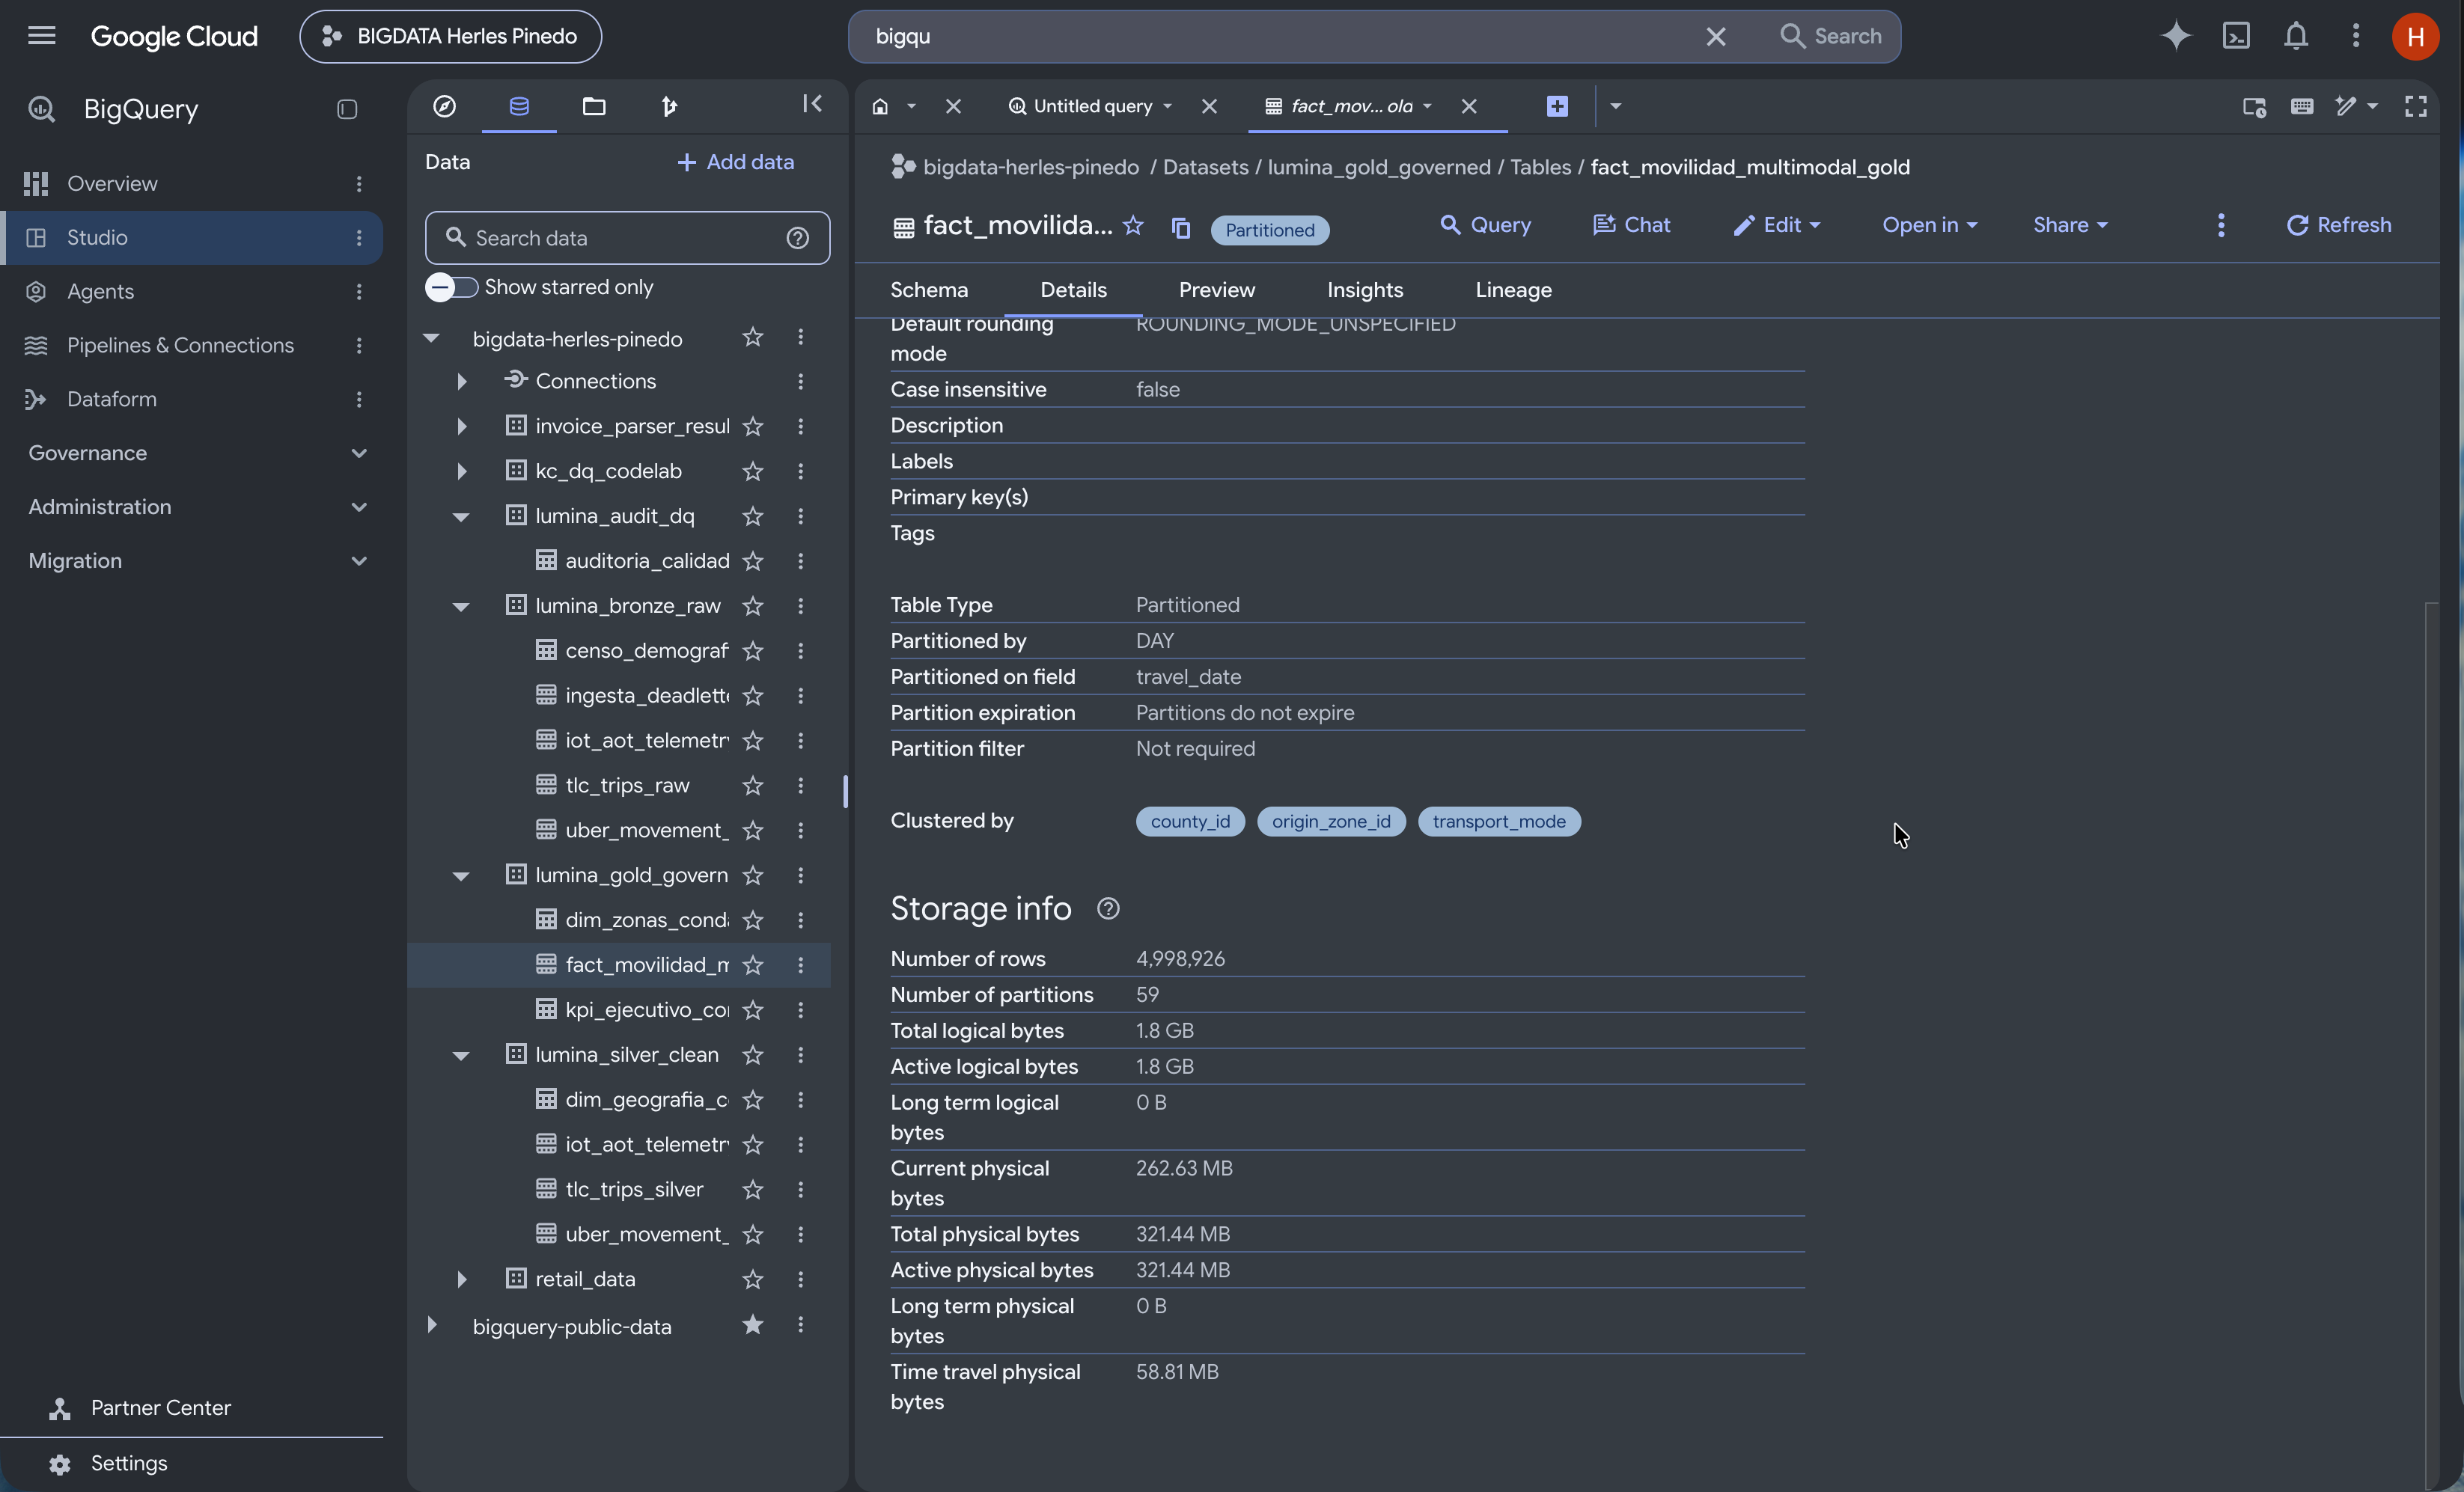
\includegraphics[width=0.9\textwidth]{Capturas de pantalla/C1.png}
  \caption{Evidencia GCP (C1): Datasets Medallion y tablas particionadas/clusterizadas creadas en BigQuery.}
\end{figure}

\begin{figure}[H]
  \centering
  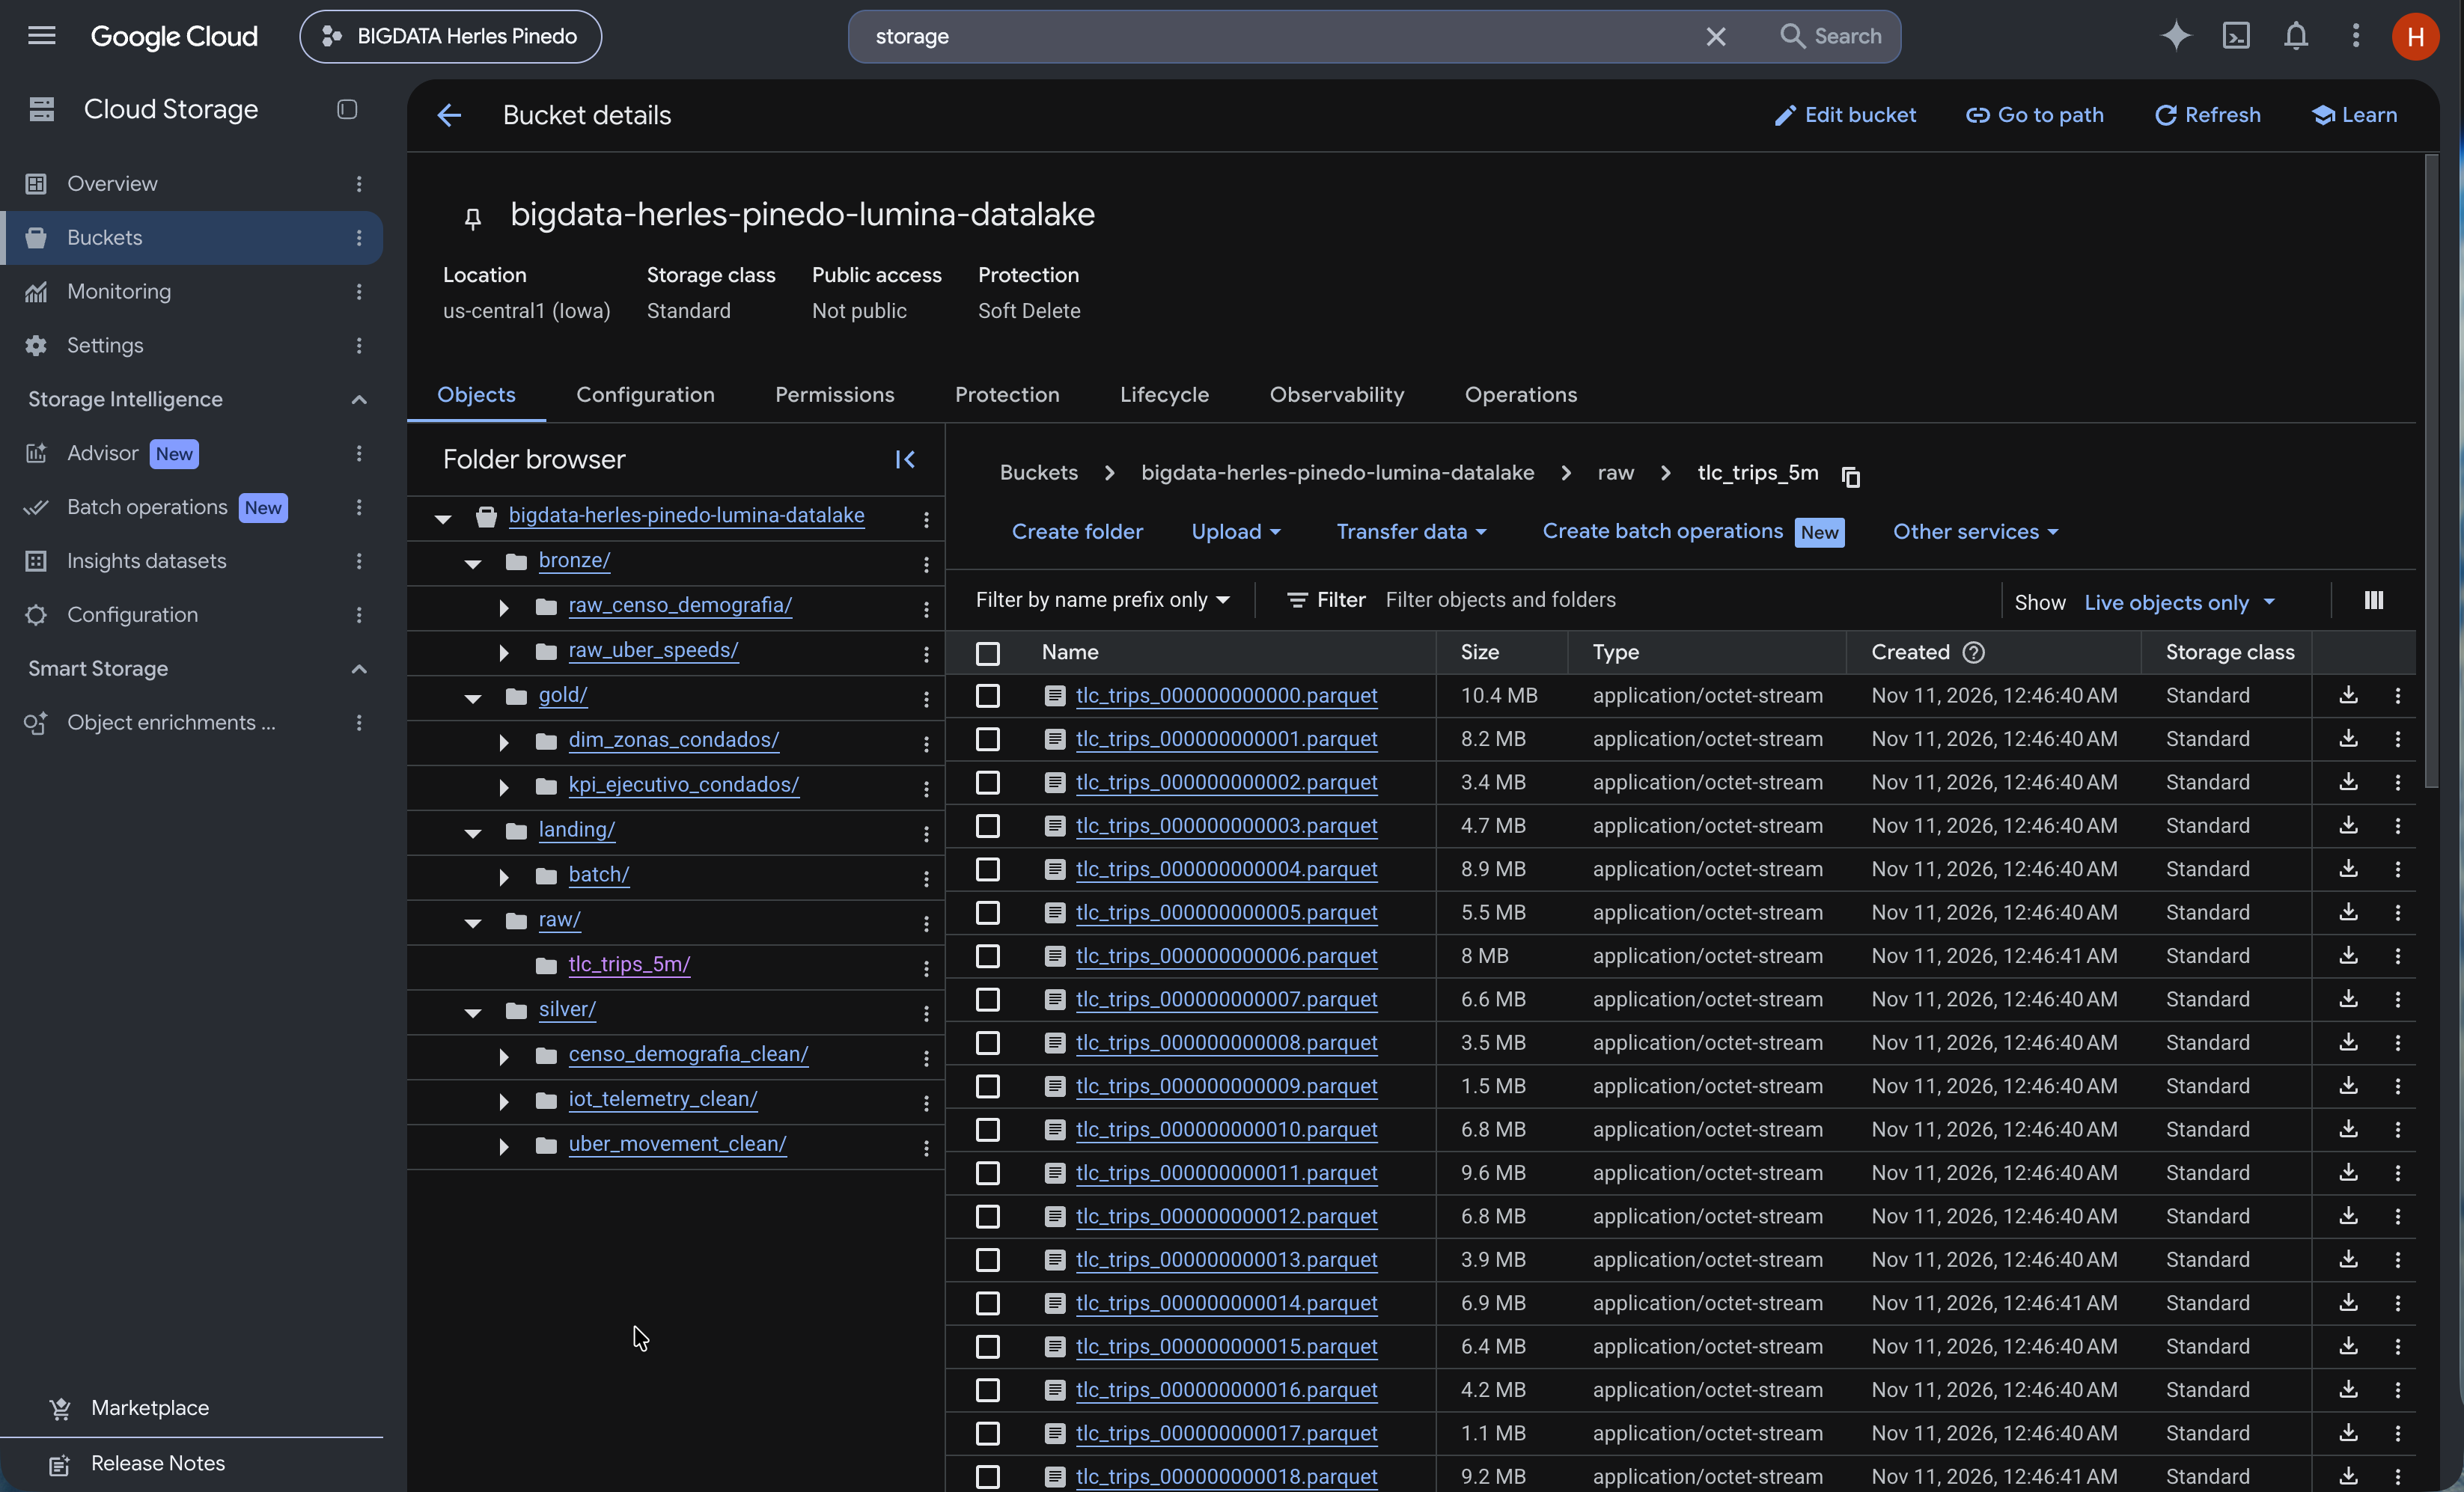
\includegraphics[width=0.9\textwidth]{Capturas de pantalla/G4.png}
  \caption{Evidencia GCP (G4): Bucket de Cloud Storage organizado en capas (\texttt{landing/}, \texttt{raw/}, \texttt{bronze/}, \texttt{silver/}, \texttt{gold/}).}
\end{figure}

% ==============================================================================
% 3. PASO 2: INGESTA BATCH MULTIFUENTE
% ==============================================================================
\section{Paso 2: Ingesta Batch Multifuente sin Sobreescritura}
\noindent\textbf{Script:} \path{Avance1_P1_Lumina_Ingesta_Storage/02_ingesta_batch_multifuente.py}

\subsection{¿Qué implementa este script?}
Sube los archivos CSV de las fuentes batch (F1 Viajes TLC, F2 Uber Movement Speeds y F4 Censo INE) a Cloud Storage (\path{landing/batch/}) y los carga en BigQuery Bronze mediante una tabla \textit{staging} temporal seguida de un \texttt{MERGE} idempotente por llave natural. Esto evita duplicados si el proceso se reintenta.

\begin{lstlisting}[language=Python,caption={Carga staging + MERGE idempotente en 02\_ingesta\_batch\_multifuente.py (líneas 271--303)}]
def cargar_csv_sin_reemplazar(local_file, table_name, merge_keys):
    stage = f"{table_name}_stage_{uuid.uuid4().hex[:12]}"
    target = f"{config.GCP_PROJECT_ID}.{config.BQ_DATASET_BRONZE}.{table_name}"
    staging = f"{config.GCP_PROJECT_ID}.{config.BQ_DATASET_BRONZE}.{stage}"
    # 1. Subir lote a GCS y cargar staging
    run_cmd(["gcloud", "storage", "cp", str(local_file), uri, ...], "Preservar lote en GCS")
    run_cmd(query_prefix + [f"CREATE TABLE `{staging}` LIKE `{target}`"], "Crear staging")
    run_cmd(["bq", "load", "--source_format=CSV", "--skip_leading_rows=1", ..., staging, uri], ...)
    # 2. MERGE idempotente con deduplicación QUALIFY
    sql = (f"MERGE `{target}` T USING (SELECT * FROM `{staging}` "
           f"QUALIFY ROW_NUMBER() OVER (PARTITION BY {partition} ORDER BY ts_ingesta_bq DESC) = 1) S "
           f"ON {on} WHEN MATCHED THEN UPDATE SET {updates} "
           f"WHEN NOT MATCHED THEN INSERT ({names}) VALUES ({values})")
    run_cmd(query_prefix + [sql], "MERGE idempotente a Bronze")
\end{lstlisting}

\begin{lstlisting}[language=bash,caption={Ejecución del Paso 2}]
python3 02_ingesta_batch_multifuente.py --upload
\end{lstlisting}

% ==============================================================================
% 4. PASO 3: STREAMING IOT + APACHE BEAM + DLQ
% ==============================================================================
\section{Paso 3: Ingesta Streaming IoT (Pub/Sub + Apache Beam + DLQ)}
\noindent\textbf{Scripts:} \path{03_simulador_streaming_iot_aot_pubsub.py} y \path{04_pipeline_streaming_beam_bq.py}

\subsection{¿Qué implementan?}
\begin{itemize}[leftmargin=1.5em]
  \item \path{03_simulador_streaming_iot_aot_pubsub.py} emite lecturas JSON de sensores Array of Things y nodos ferroviarios OART al tópico Pub/Sub.
  \item \path{04_pipeline_streaming_beam_bq.py} (apoyado en \path{telemetry.py}) valida reglas físicas (vibración, temperatura, timestamp válido). Los eventos válidos ingresan a \path{bronze_iot_aot_stream}; los corruptos se aíslan en la Dead-Letter Queue (\path{bronze_deadletter_dlq}).
\end{itemize}

\begin{lstlisting}[language=bash,caption={Ejecución de productor y pipeline streaming}]
# 1. Publicar eventos IoT de prueba en Pub/Sub
python3 03_simulador_streaming_iot_aot_pubsub.py --max-messages 50 --interval 0.3

# 2. Consumir desde Pub/Sub y enrutar válidos vs DLQ hacia BigQuery Bronze
python3 04_pipeline_streaming_beam_bq.py
\end{lstlisting}

\begin{figure}[H]
  \centering
  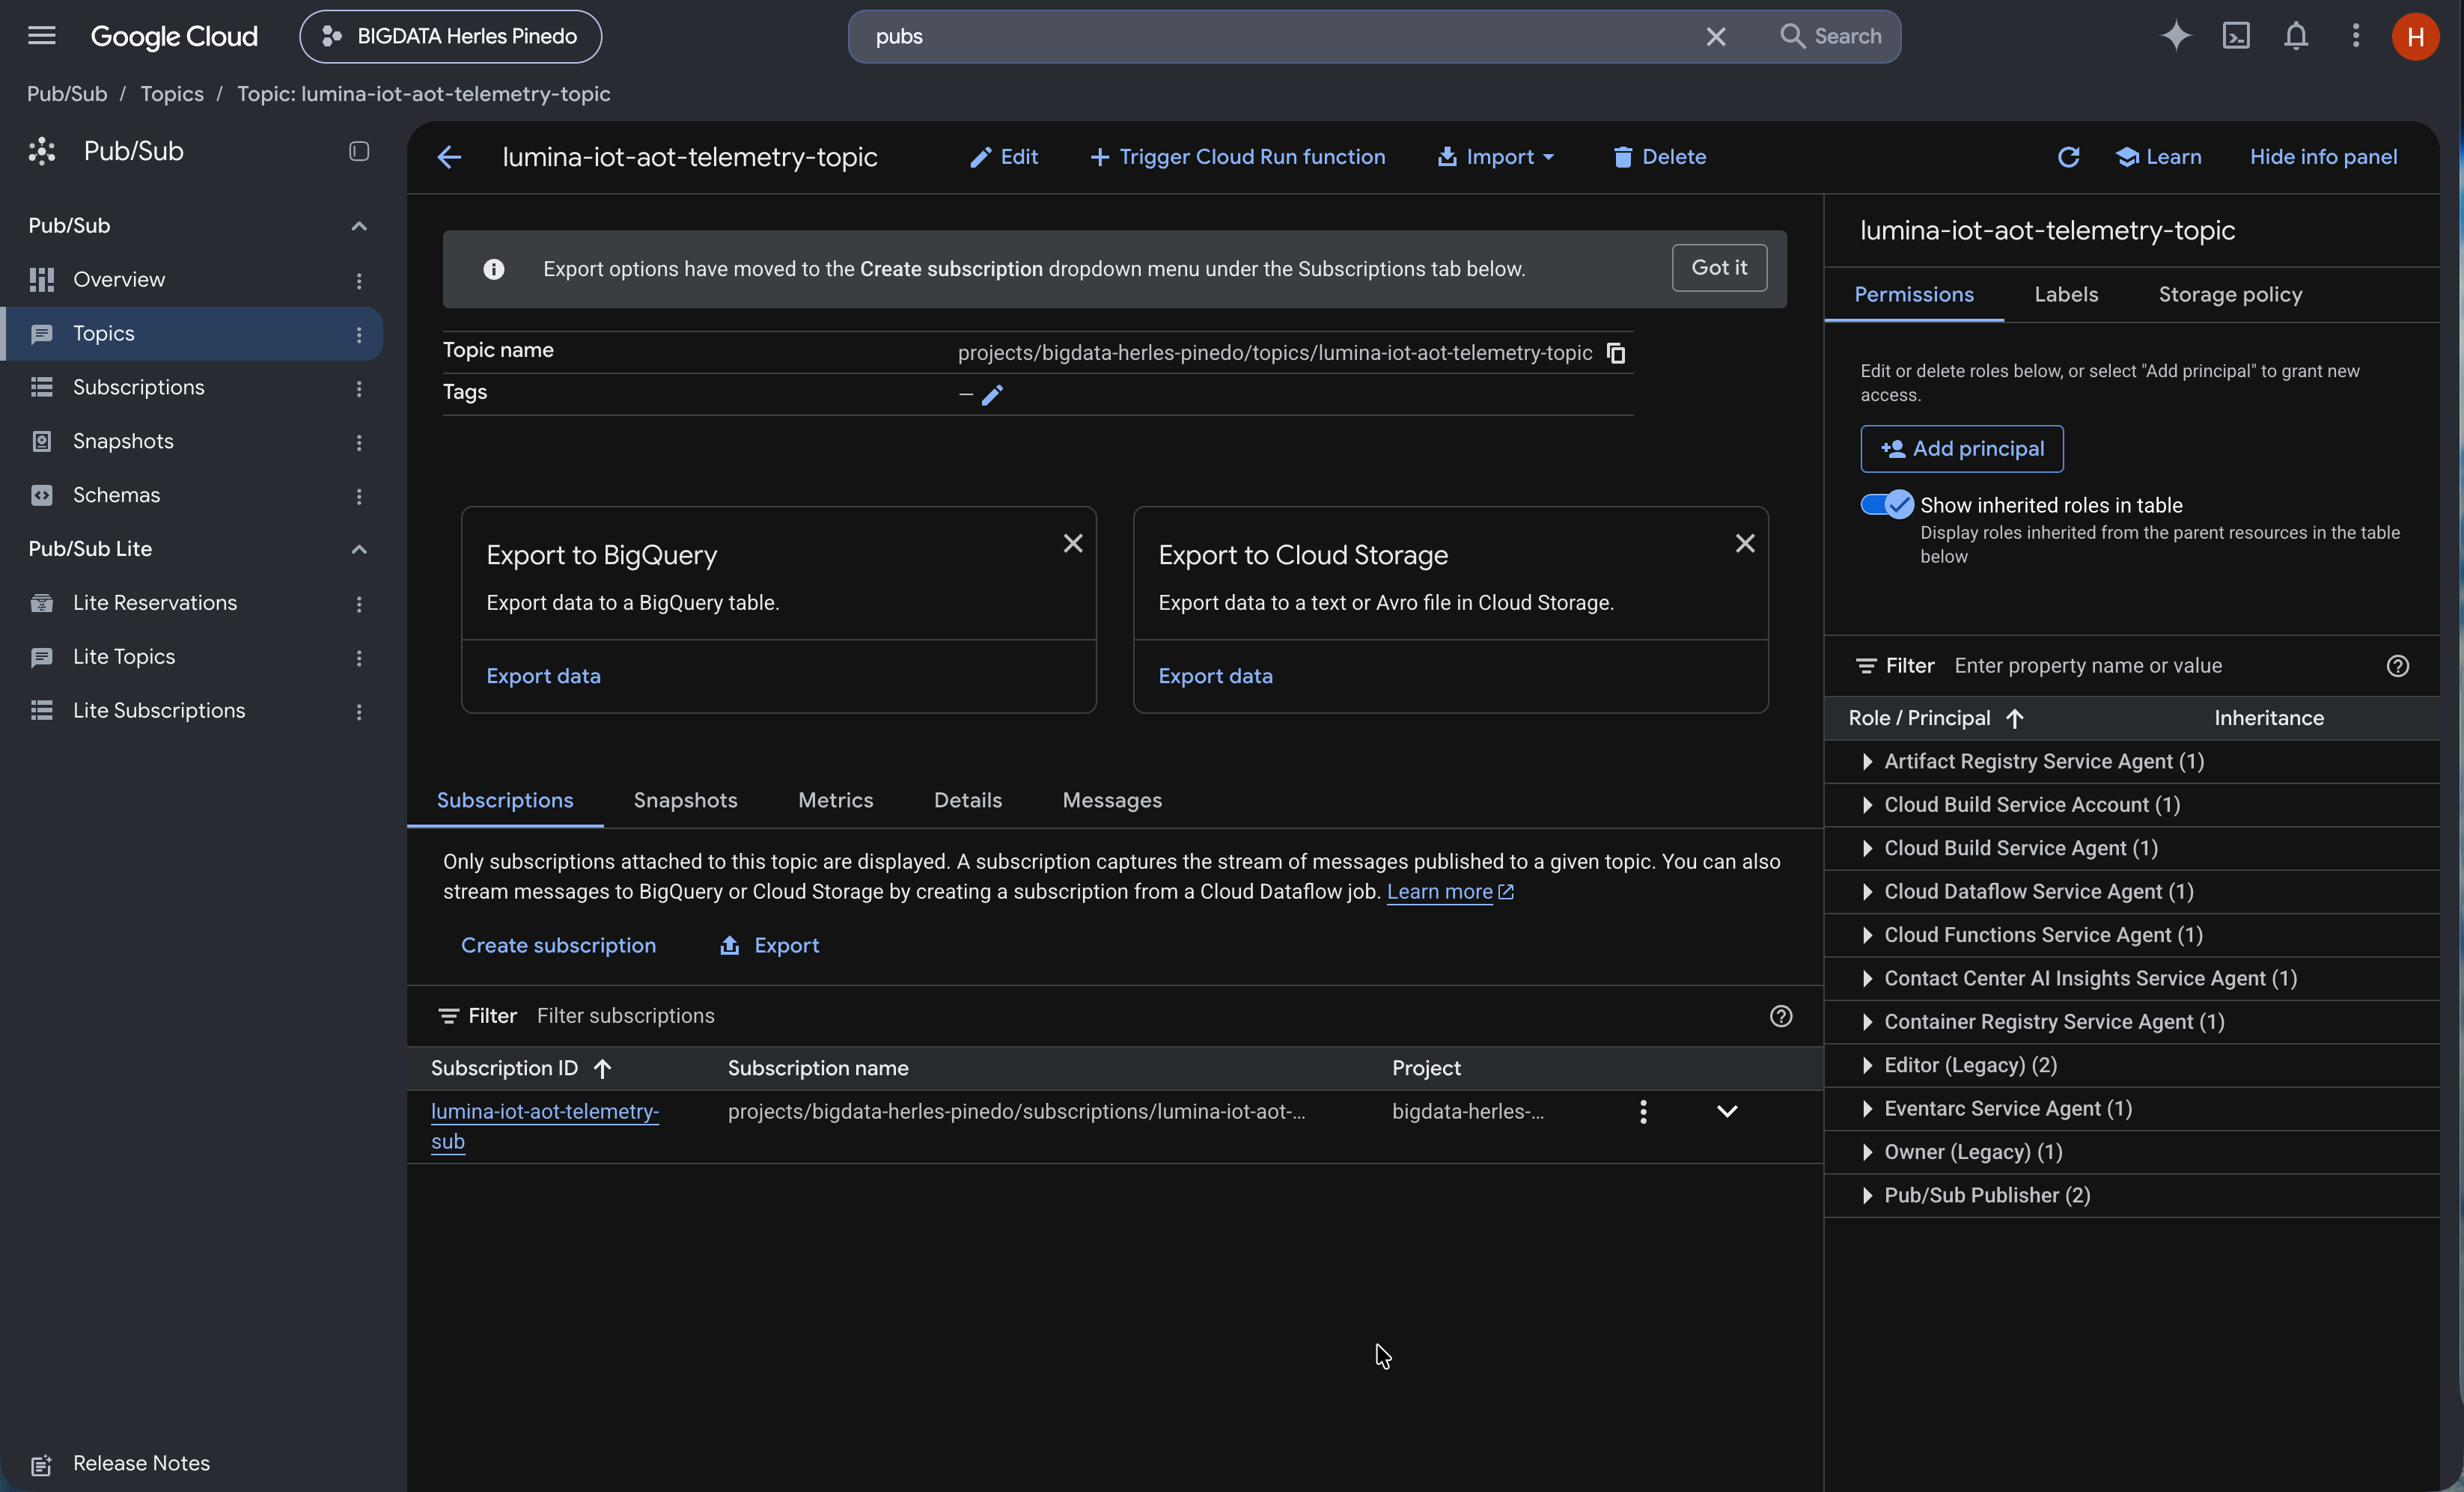
\includegraphics[width=0.9\textwidth]{Capturas de pantalla/C3.png}
  \caption{Evidencia GCP (C3): Tópico y suscripción activos en Cloud Pub/Sub recibiendo telemetría IoT.}
\end{figure}

% ==============================================================================
% 5. PASO 4: PROCESAMIENTO MEDALLION SILVER -> DQ -> GOLD
% ==============================================================================
\section{Paso 4: Procesamiento Medallion (Silver a Gold con Compuerta DQ)}
\noindent\textbf{Scripts:} \path{06_pipeline_medallion_silver_gold_ml.py}, \path{pipeline_sql.py} y \path{06b_pipeline_pyspark_dataproc_silver_gold.py}

\subsection{¿Qué implementa este paso?}
El orquestador SQL ejecuta cuatro etapas secuenciales con compuerta de calidad obligatoria:
\begin{enumerate}[leftmargin=1.5em]
  \item \textbf{Bronze $\rightarrow$ Silver (\path{build_silver_sql}):} limpia nulos, normaliza zonas y deduplica por \path{QUALIFY ROW_NUMBER() OVER (PARTITION BY trip_id ...)}.
  \item \textbf{Auditoría SQL (\path{build_dq_sql}):} evalúa reglas de integridad y SLA en \path{lumina_governance_audit}.
  \item \textbf{Compuerta de Calidad (\path{build_quality_gate_sql}):} aborta el pipeline si alguna regla crítica cae por debajo del umbral SLA.
  \item \textbf{Silver $\rightarrow$ Gold (\path{build_gold_sql}):} construye la dimensión \path{dim_zonas_condados_gold}, la tabla de hechos \path{fact_movilidad_multimodal_gold} (cruce exacto por fecha, hora, zona y estación OART) y el data mart ejecutivo \path{kpi_ejecutivo_condados_gold}.
\end{enumerate}

\begin{lstlisting}[language=Python,caption={Secuencia controlada con compuerta DQ en 06\_pipeline\_medallion\_silver\_gold\_ml.py}]
def construir_capas_silver_y_gold():
    client = bigquery.Client(project=config.GCP_PROJECT_ID)
    for title, builder in (("Bronze -> Silver", build_silver_sql),
                           ("Auditoría SQL", build_dq_sql),
                           ("Compuerta de calidad", build_quality_gate_sql),
                           ("Silver -> Gold", build_gold_sql)):
        ejecutar_sql(client, title, builder())
    exportar_cache_frontend(client)
\end{lstlisting}

\begin{lstlisting}[language=bash,caption={Ejecución del pipeline SQL y variante PySpark}]
# Pipeline Medallion completo en BigQuery
python3 06_pipeline_medallion_silver_gold_ml.py

# Procesamiento distribuido en PySpark (local o Dataproc Serverless)
python3 06b_pipeline_pyspark_dataproc_silver_gold.py
\end{lstlisting}

\begin{figure}[H]
  \centering
  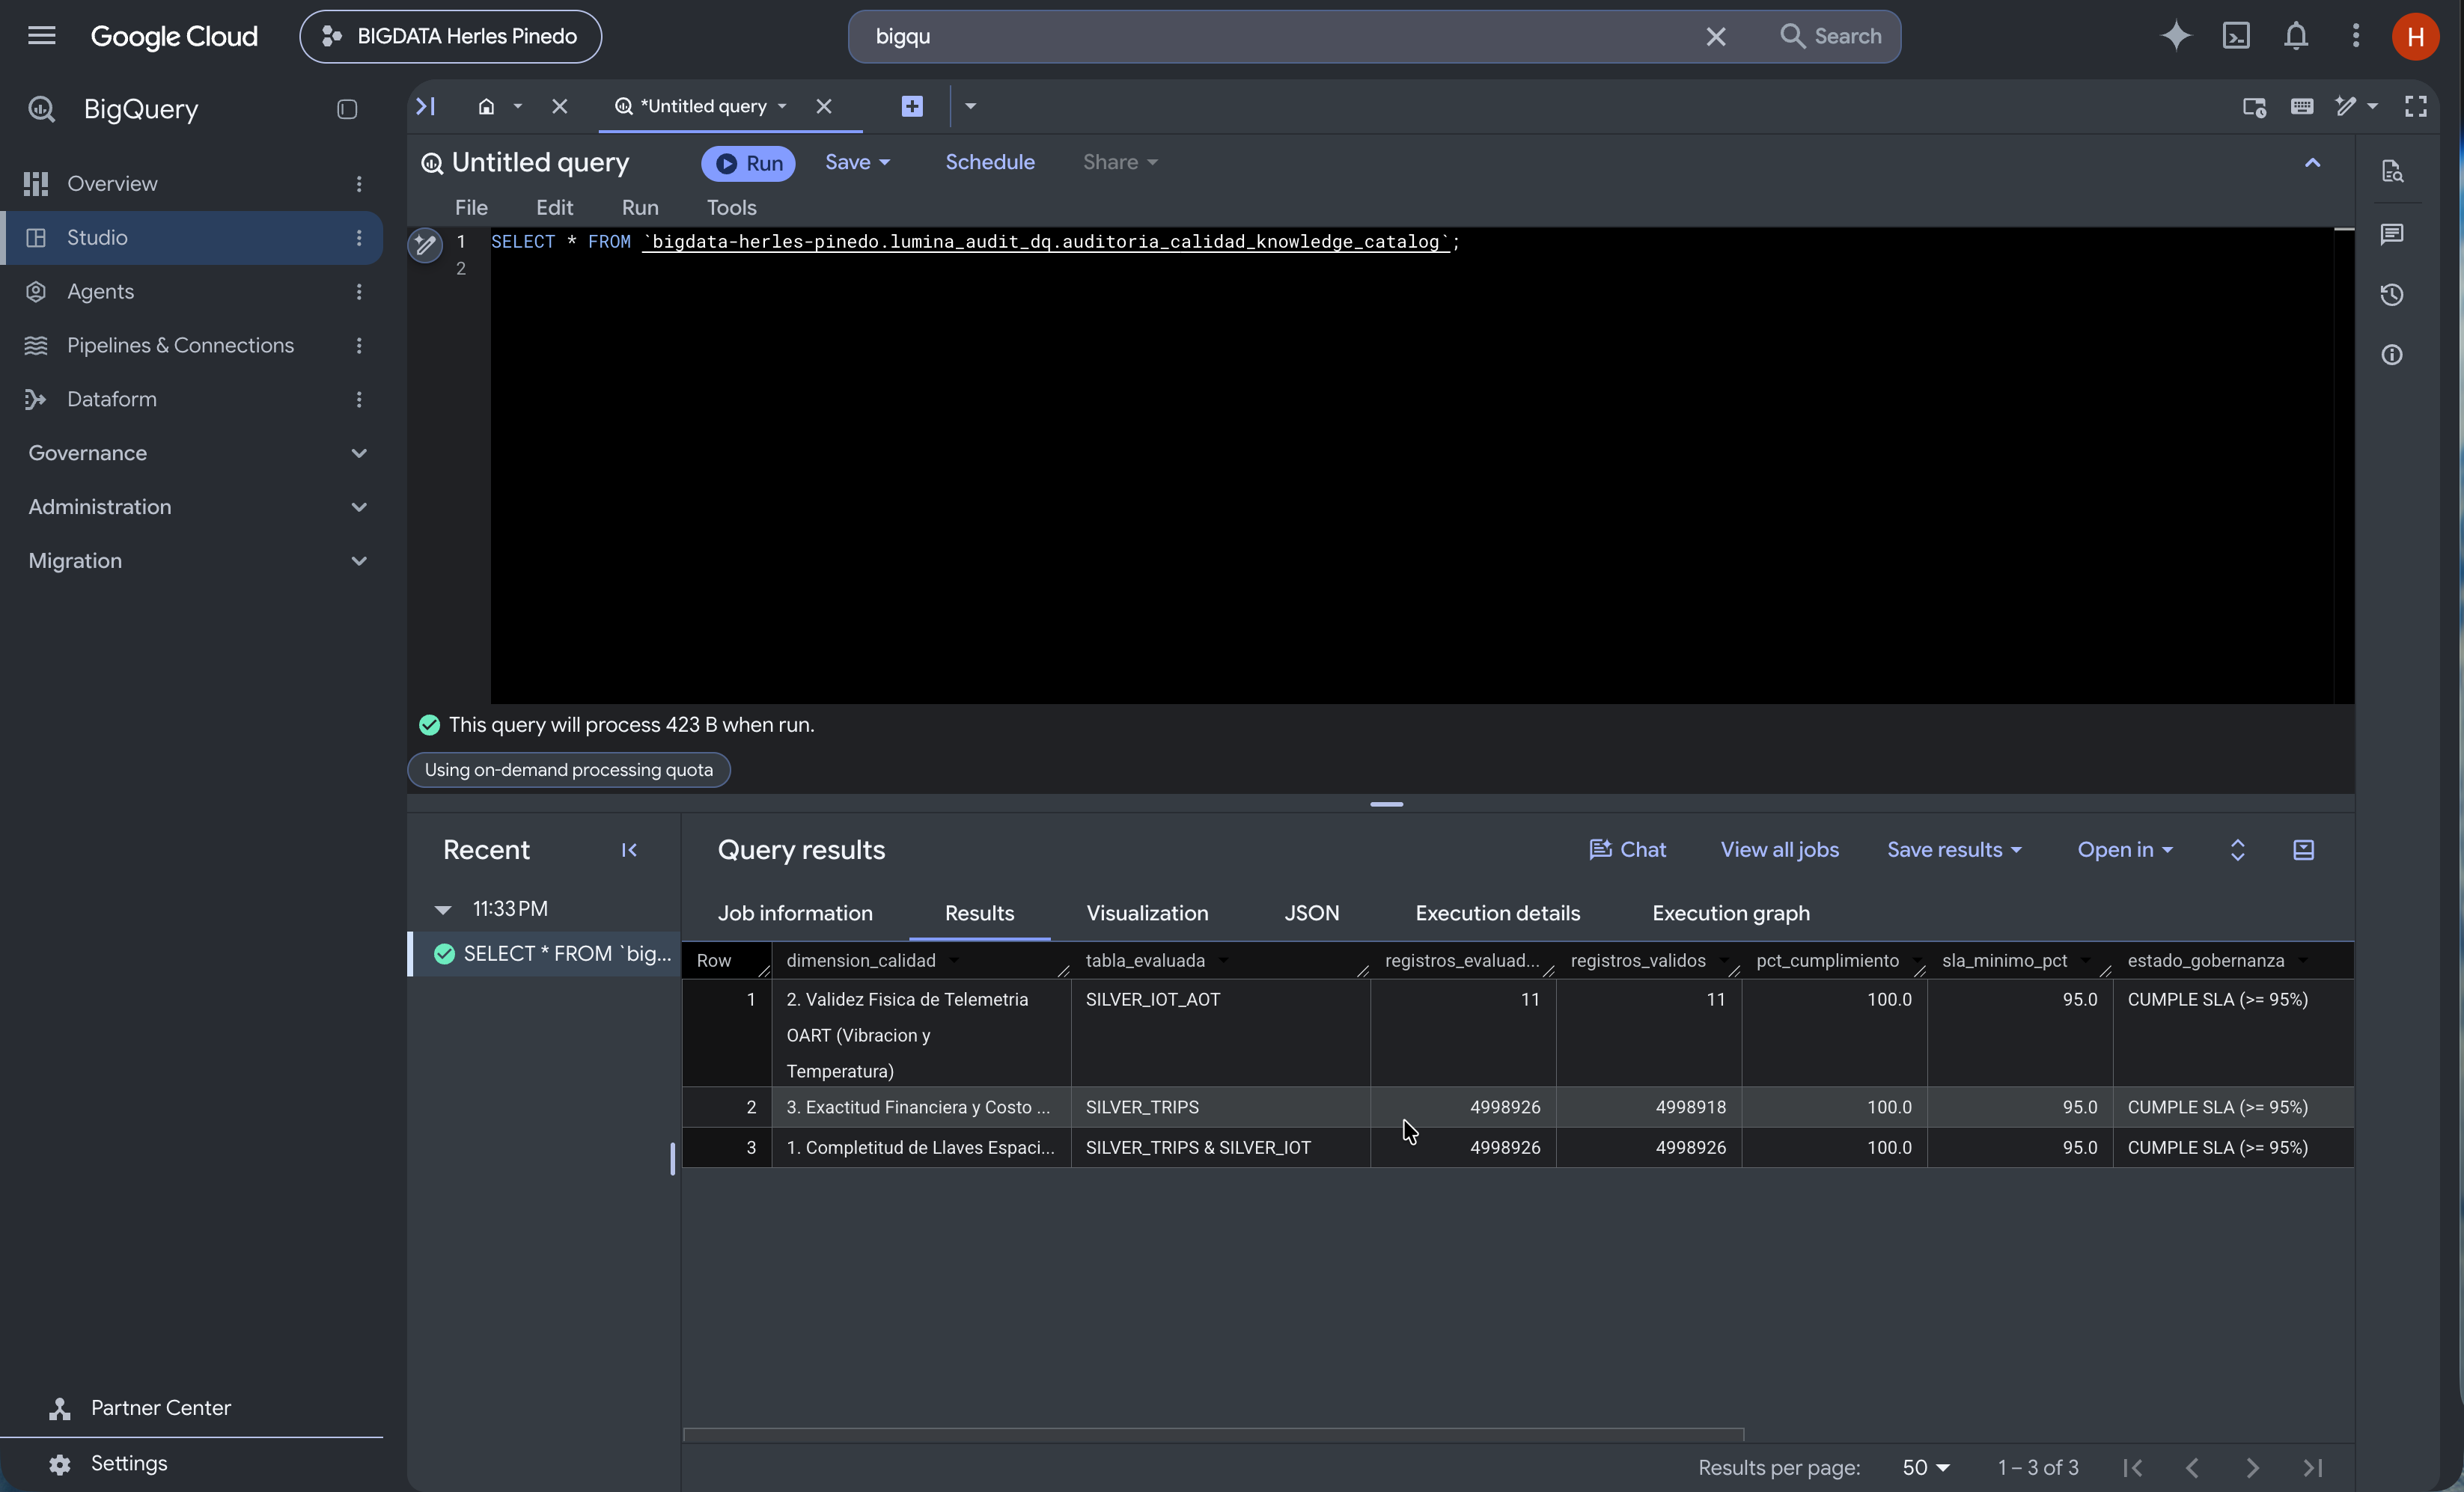
\includegraphics[width=0.9\textwidth]{Capturas de pantalla/C2.png}
  \caption{Evidencia GCP (C2): Resultados de auditoría de calidad (DQ) en BigQuery superando el SLA.}
\end{figure}

\begin{figure}[H]
  \centering
  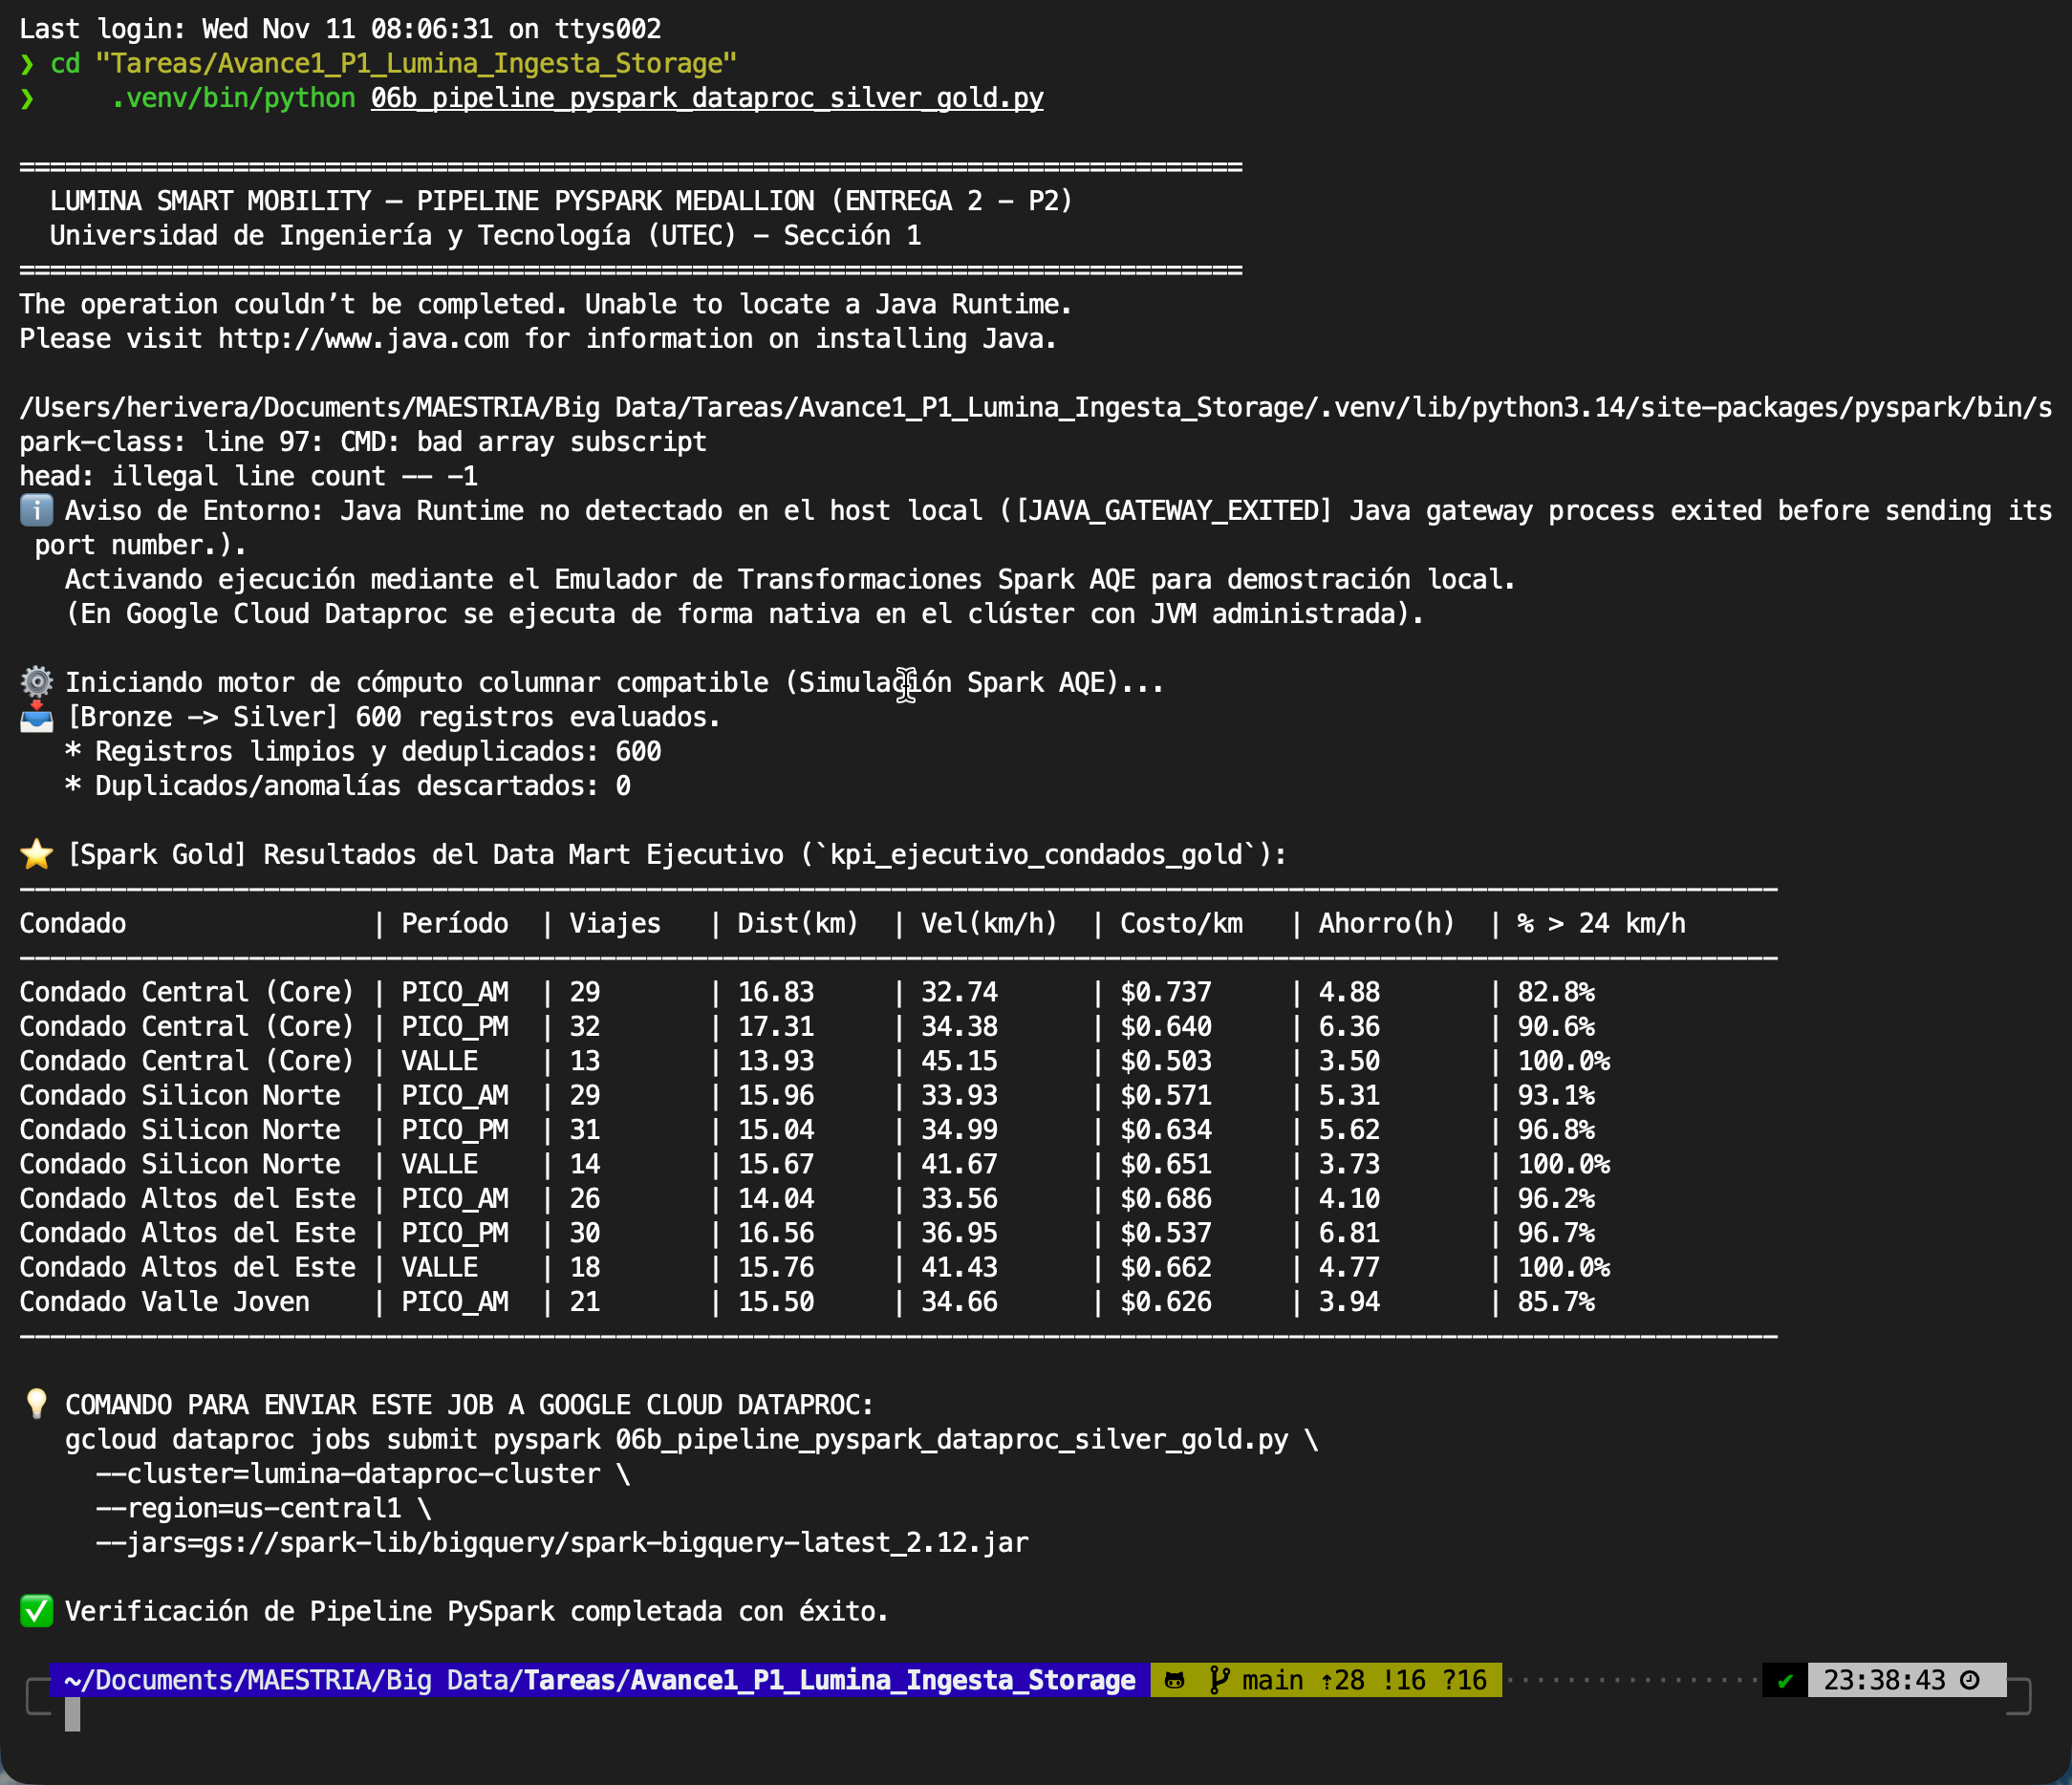
\includegraphics[width=0.9\textwidth]{Capturas de pantalla/G5.png}
  \caption{Evidencia de ejecución PySpark (G5): Procesamiento distribuido con Adaptive Query Execution (AQE).}
\end{figure}

% ==============================================================================
% 6. PASO 5: ORQUESTACIÓN CON AIRFLOW / CLOUD COMPOSER
% ==============================================================================
\section{Paso 5: Orquestación Automatizada (Airflow / Cloud Composer)}
\noindent\textbf{Script:} \path{Avance1_P1_Lumina_Ingesta_Storage/07_dag_managed_airflow_composer.py}

Para operar diariamente en producción (\texttt{04:00 AM America/Lima}), se define el DAG \path{lumina_medallion_end_to_end_dag} usando \path{BigQueryInsertJobOperator} con las mismas funciones SQL de \path{pipeline_sql.py}:

\begin{lstlisting}[language=Python,caption={Definición del DAG en 07\_dag\_managed\_airflow\_composer.py (líneas 26--50)}]
with DAG(
    dag_id="lumina_medallion_end_to_end_dag",
    schedule_interval="0 4 * * *",
    start_date=pendulum.datetime(2026, 1, 1, tz="America/Lima"),
    catchup=False,
    max_active_runs=1,
    ...
) as dag:
    tasks = []
    for task_id, builder in (
        ("transicion_bronze_a_silver", build_silver_sql),
        ("auditoria_sql_calidad", build_dq_sql),
        ("bloquear_publicacion_si_falla_sla", build_quality_gate_sql),
        ("transicion_silver_a_gold_estrella", build_gold_sql),
    ):
        task = BigQueryInsertJobOperator(
            task_id=task_id, project_id=config.GCP_PROJECT_ID, location=config.GCP_LOCATION,
            configuration={"query": {"query": builder(), "useLegacySql": False}},
        )
        if tasks:
            tasks[-1] >> task
        tasks.append(task)
\end{lstlisting}

% ==============================================================================
% 7. PASO 6: EXPOSICIÓN OLAP, API REST Y APLICACIÓN WEB
% ==============================================================================
\section{Paso 6: Exposición OLAP, API REST y Aplicación Web (P3)}
\noindent\textbf{Scripts:} \path{P3/usar_datos_existentes.py}, \path{P3/recuperar_web_pasajero.py}, \path{08_app_exposicion_frontend_lumina.py} y \path{frontend/}

\subsection{Exportación de agregados Gold verificados}
Antes de levantar la web, se ejecutan los scripts de lectura sobre \path{fact_movilidad_multimodal_gold} (\texttt{5,006,606} registros, 24 zonas \path{ZDL-001}--\path{ZDL-024}) para generar las evidencias JSON consumidas por la API:
\begin{lstlisting}[language=bash,caption={Exportación de métricas OLAP y trayectos desde BigQuery Gold}]
python3 P3/usar_datos_existentes.py
python3 P3/recuperar_web_pasajero.py
\end{lstlisting}

\subsection{Compilación del frontend React y arranque de servidores}
\begin{lstlisting}[language=bash,caption={Build de React y arranque de APIs Python (8080) y Node (3000)}]
# 1. Compilar interfaz React e incrustar en plantilla Flask (templates/p3_olap.html)
cd frontend && npm install && npm run build

# 2. Iniciar servidor Node (puerto 3000) o servidor Flask (puerto 8080)
npm start                                           # http://127.0.0.1:3000/p3
cd ../Avance1_P1_Lumina_Ingesta_Storage
python3 08_app_exposicion_frontend_lumina.py        # http://127.0.0.1:8080/p3
\end{lstlisting}

\subsection{Endpoints expuestos por la plataforma}
\begin{table}[H]
  \centering
  \small
  \begin{tabularx}{\textwidth}{@{}>{\raggedright\arraybackslash}p{4.3cm}XX@{}}
    \toprule
    \textbf{Método y Ruta} & \textbf{Descripción} & \textbf{Fuente} \\
    \midrule
    \path{GET /p3} & Aplicación web del pasajero + Panel Analítico & React (\path{p3_olap.html}) \\
    \path{GET /api/v1/olap-kpis} & KPIs agregados OLAP, desglose por modo y SQL & \path{datos_existentes_latest.json} \\
    \path{GET /api/v1/passenger-data} & 2,880 grupos de trayectos (24$\times$24$\times$5) y ejemplos & \path{movilidad_pasajero_latest.json} \\
    \path{GET /api/v1/health} & Healthcheck para balanceador / Cloud Run & Estado del servicio \\
    \bottomrule
  \end{tabularx}
  \caption{Contratos HTTP expuestos por la capa de servicio.}
\end{table}

\subsection{Evidencias reales del sistema en funcionamiento}

\begin{figure}[H]
  \centering
  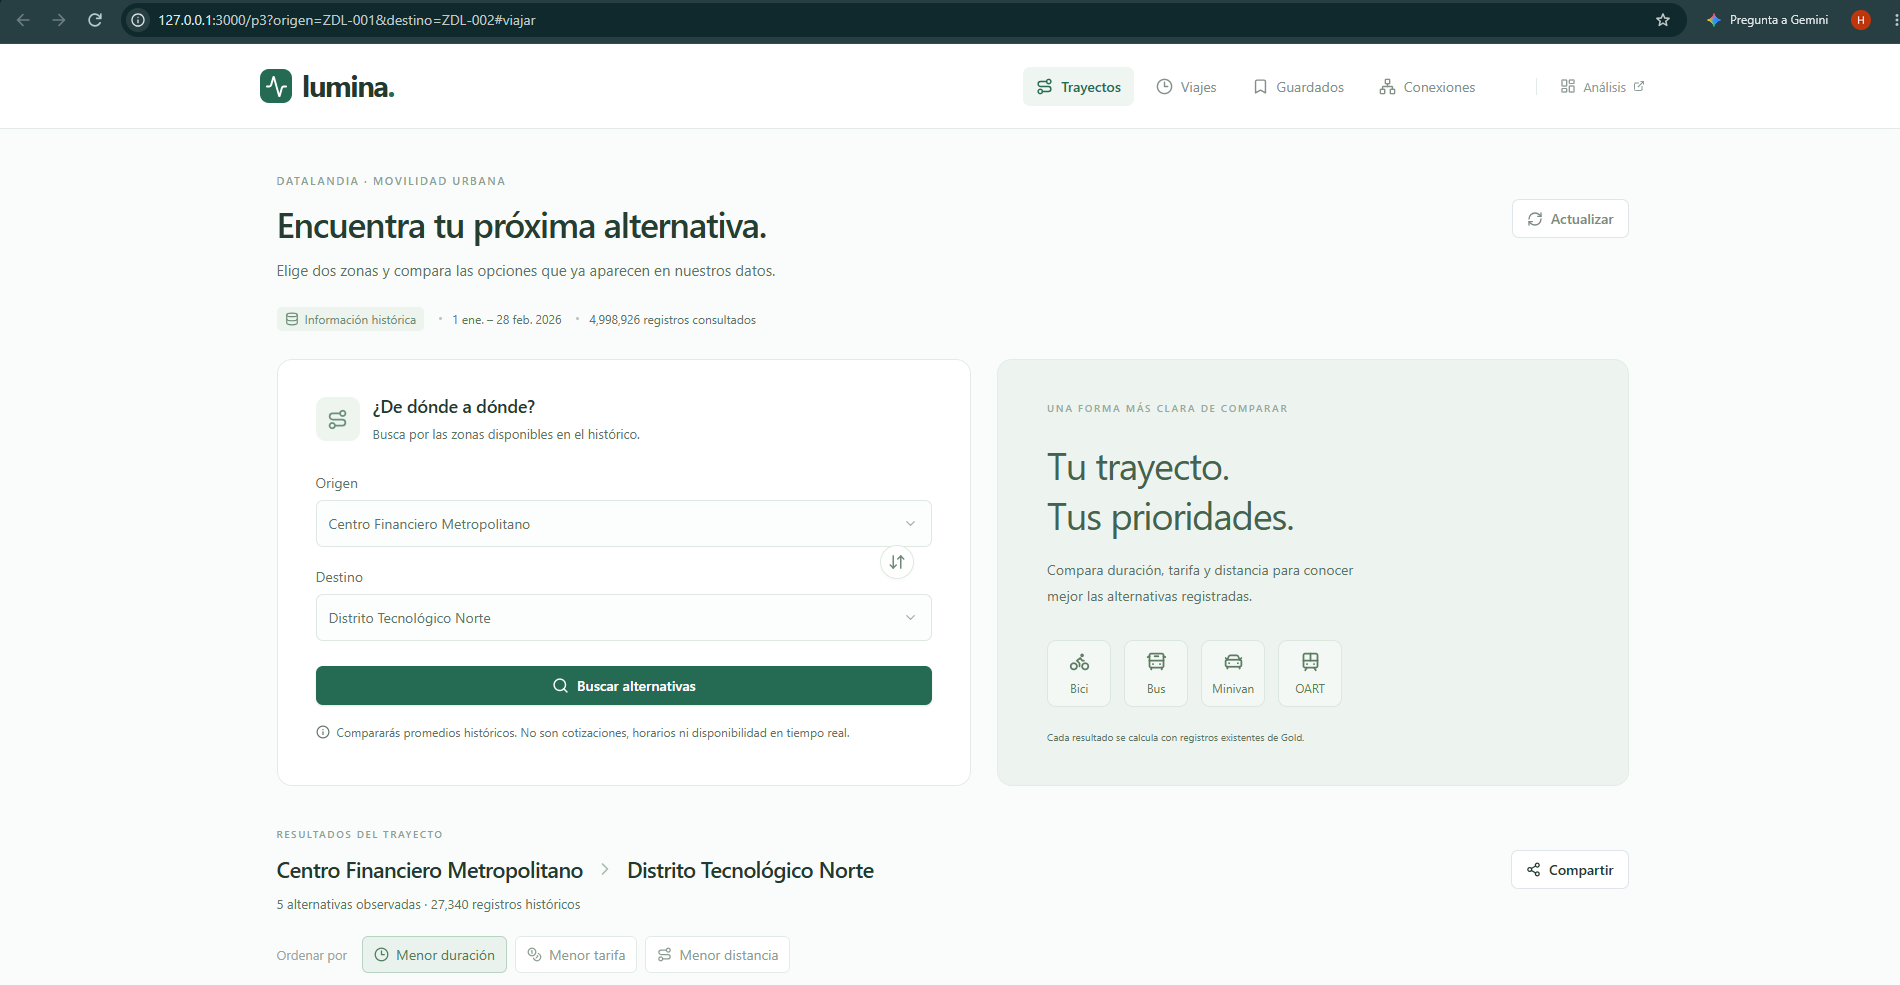
\includegraphics[width=0.9\textwidth]{P3/entrega/capturas/01-viajes.png}
  \caption{Web del pasajero en funcionamiento: búsqueda por origen/destino, comparación de alternativas y desglose por modo.}
\end{figure}

\begin{figure}[H]
  \centering
  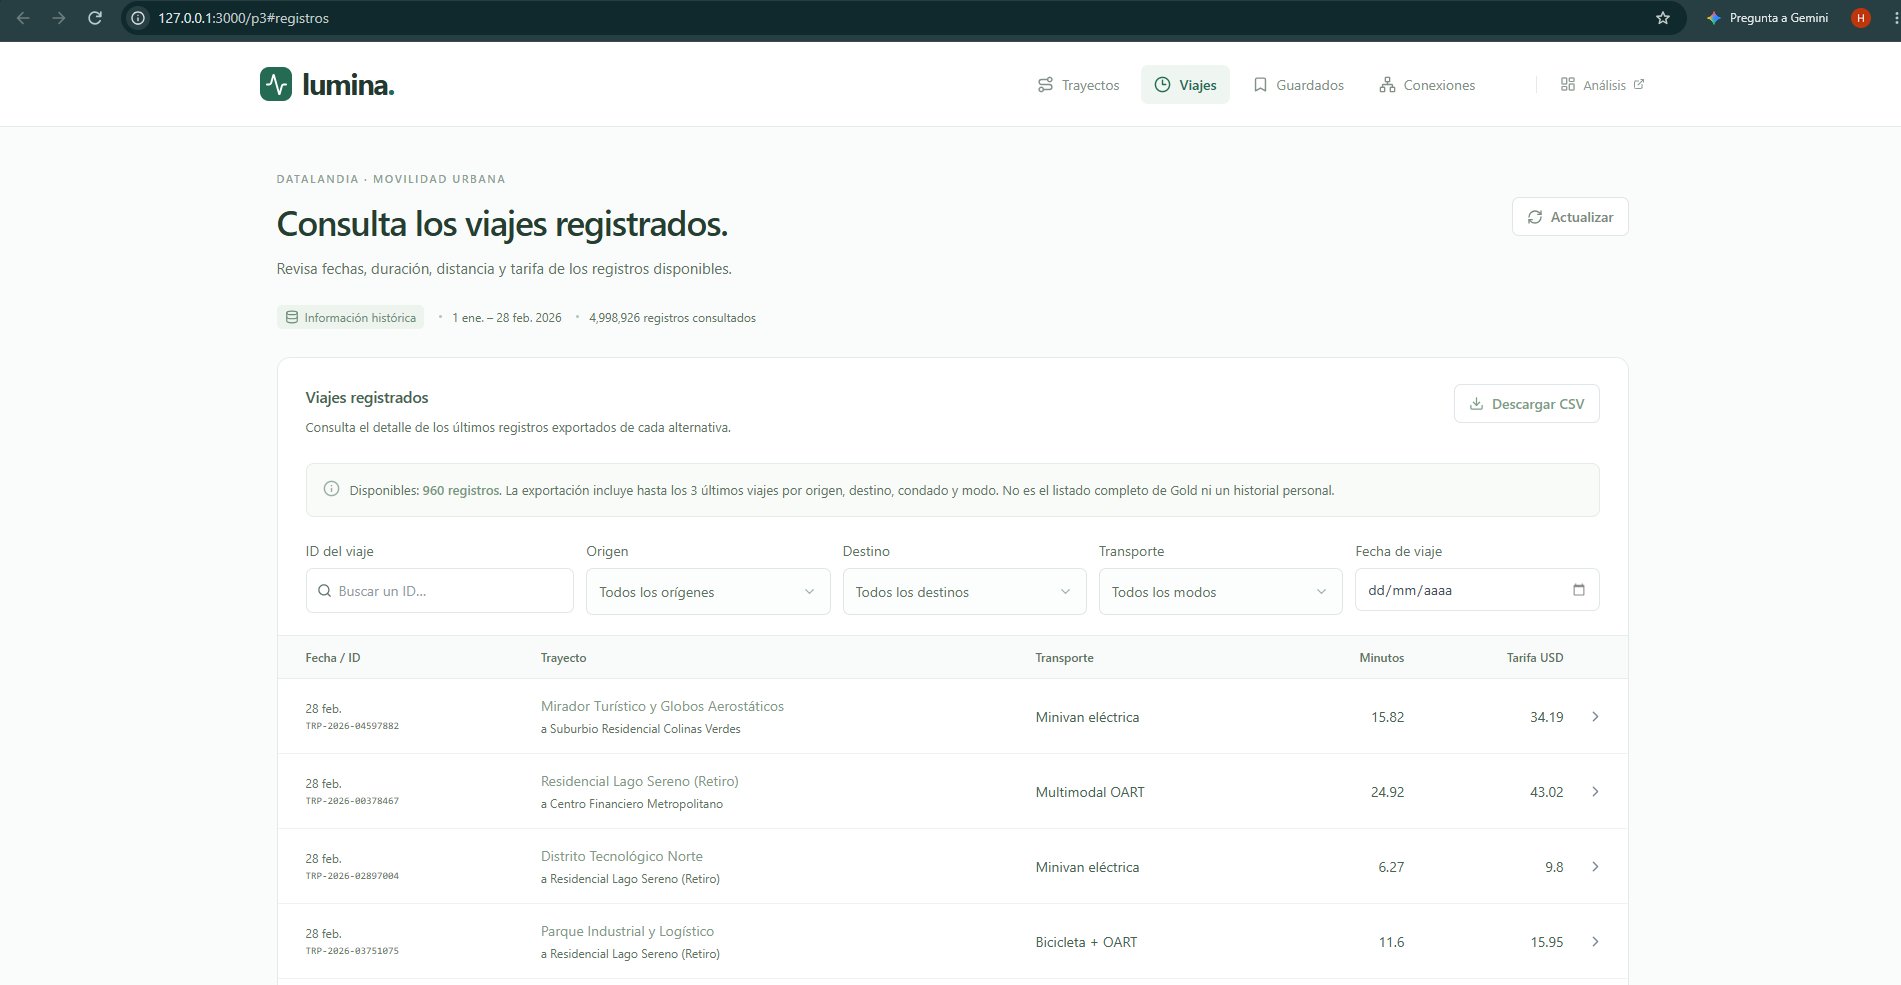
\includegraphics[width=0.9\textwidth]{P3/entrega/capturas/02-registros.png}
  \caption{Explorador de viajes registrados con filtros por zona, modo, fecha y exportación CSV con trazabilidad de \texttt{job\_id}.}
\end{figure}

\begin{figure}[H]
  \centering
  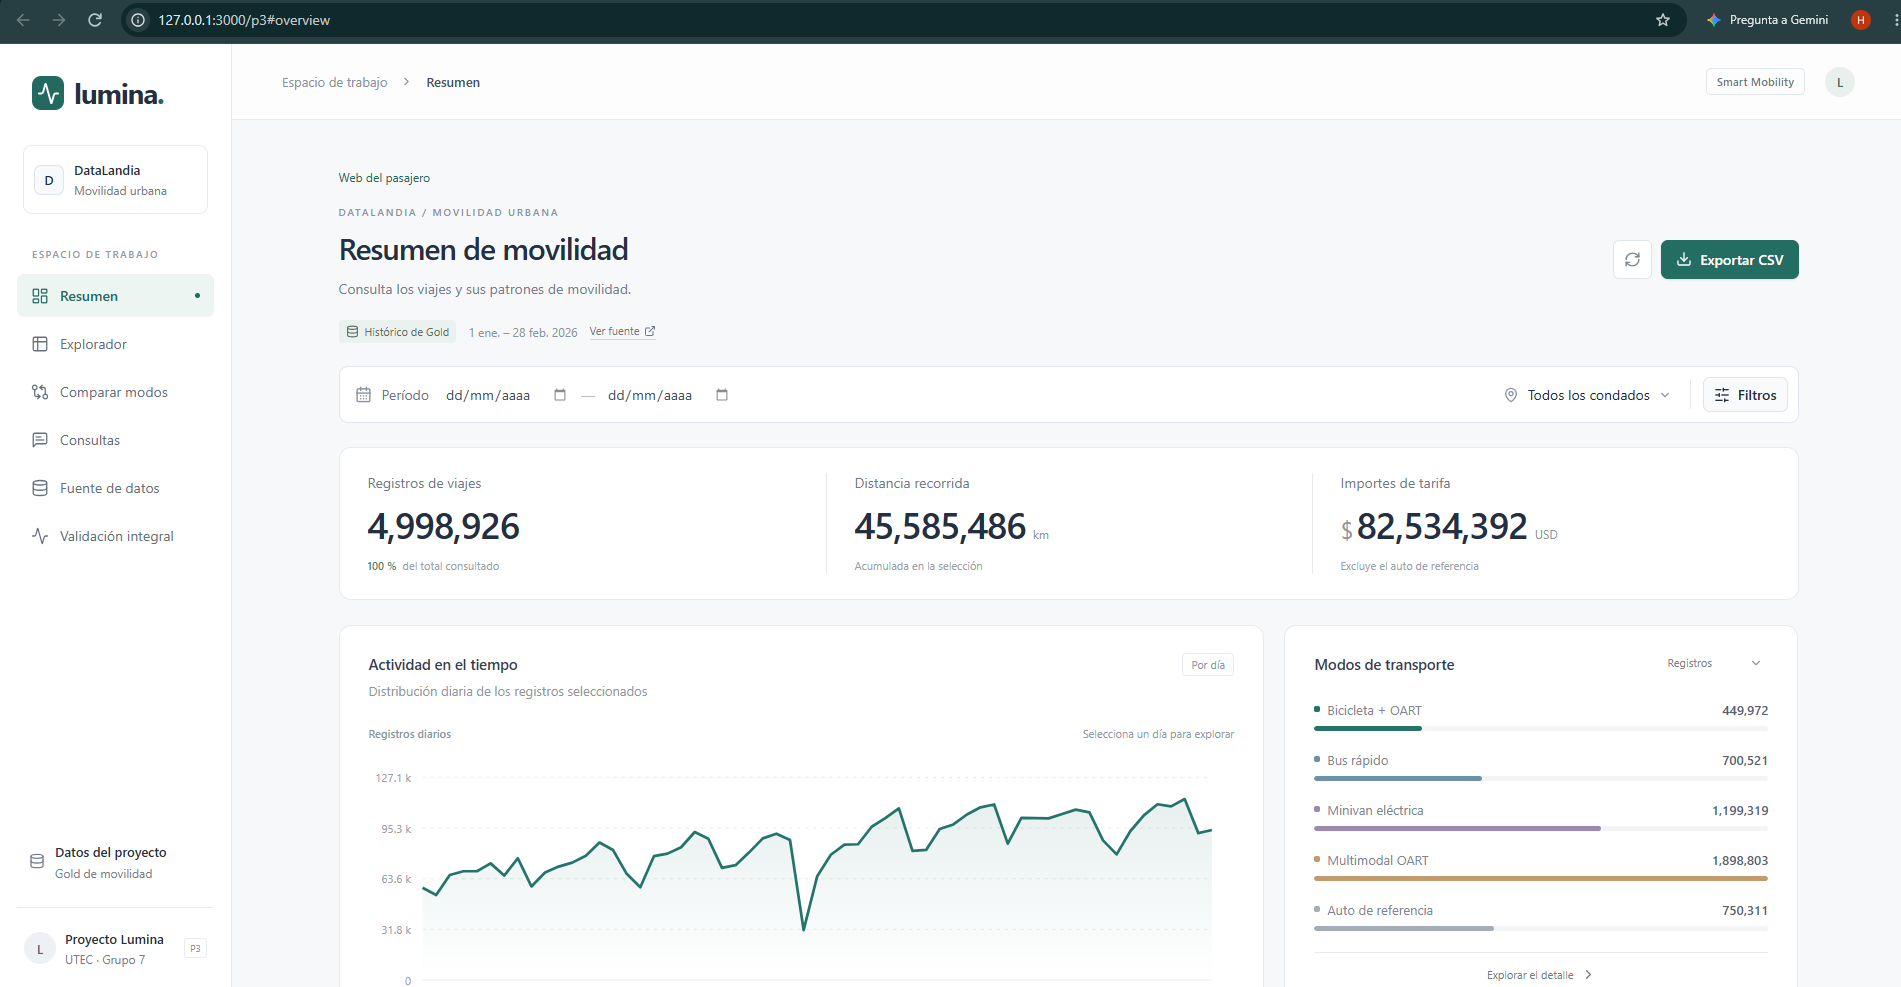
\includegraphics[width=0.9\textwidth]{P3/entrega/capturas/03-tablero.png}
  \caption{Tablero analítico OLAP (\texttt{\#overview}): evolución temporal, distribución por modo, hora y condado.}
\end{figure}

\begin{figure}[H]
  \centering
  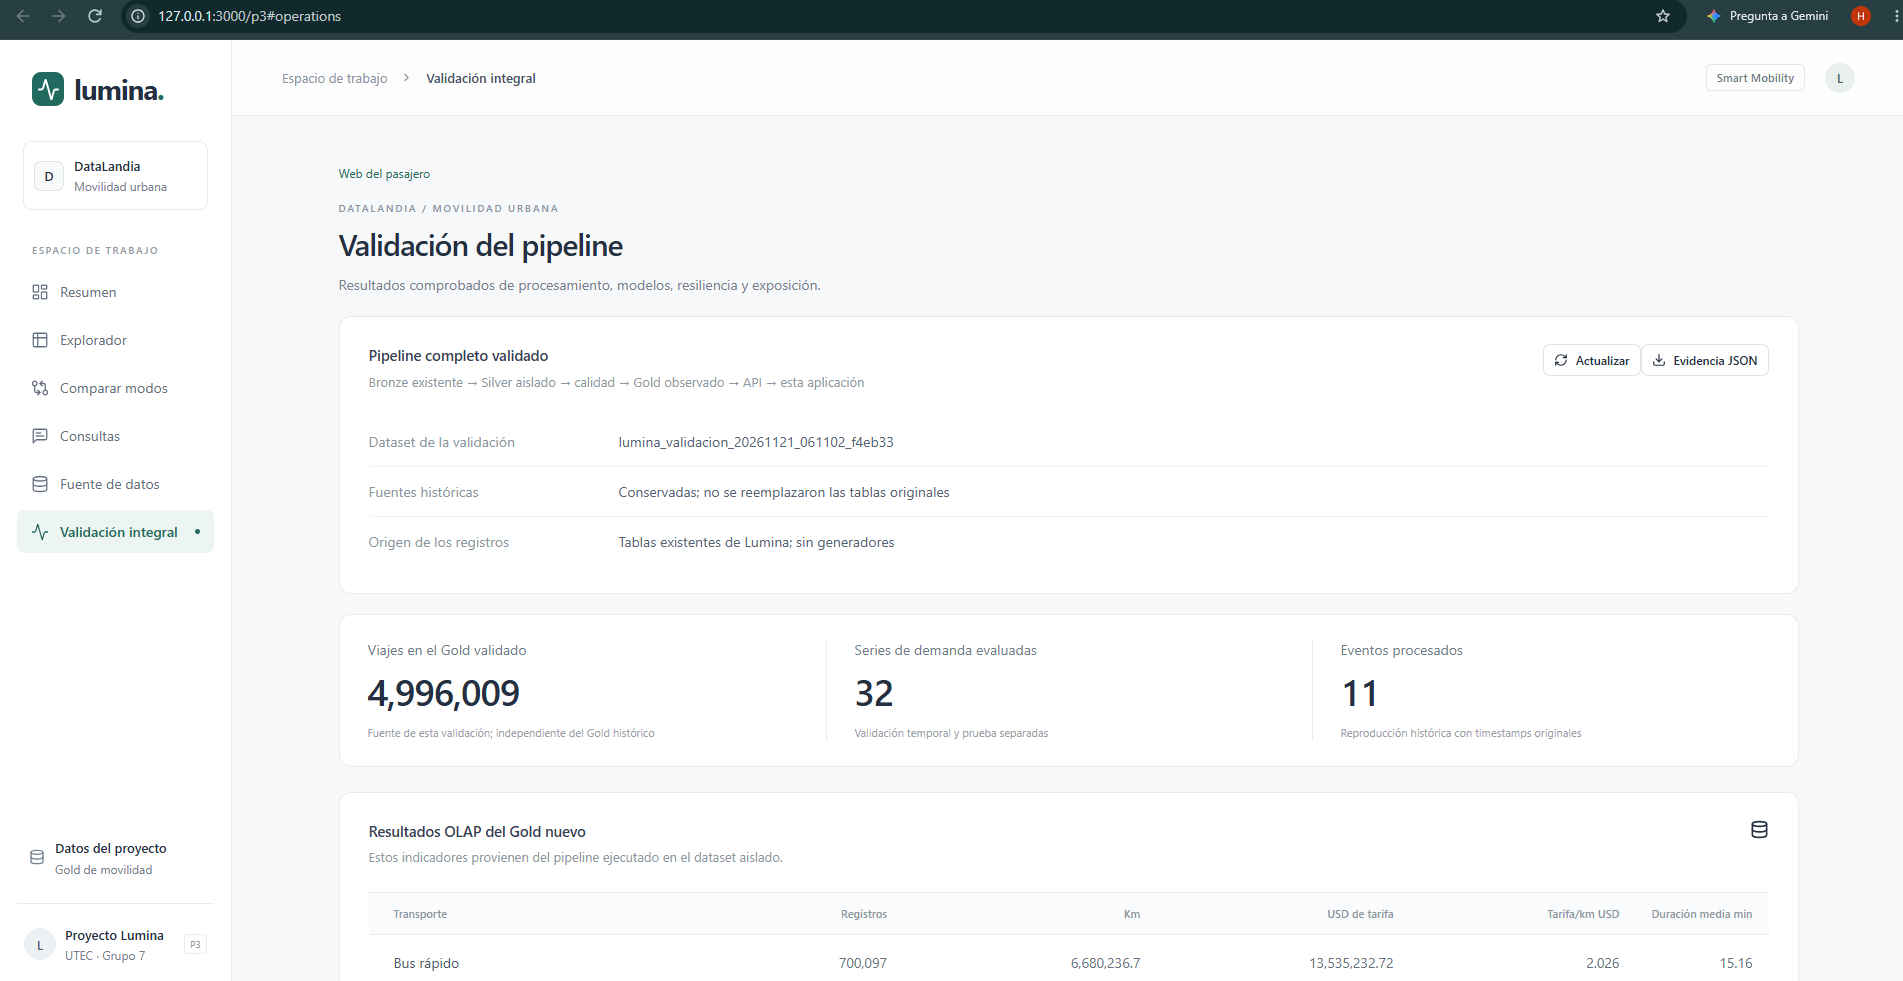
\includegraphics[width=0.9\textwidth]{P3/entrega/capturas/04-validacion.png}
  \caption{Pestaña de fuente y validación: métricas reales de BigQuery Gold, calidad de datos y esquema verificado.}
\end{figure}

% ==============================================================================
% 8. VERIFICACIÓN Y PRUEBAS AUTOMATIZADAS
% ==============================================================================
\section{Paso 7: Verificación Final y Pruebas Automatizadas}

Para certificar que la instalación del cliente quedó operativa sin regresiones ni datos fabricados, se ejecutan las dos suites de pruebas incluidas en el repositorio:

\begin{lstlisting}[language=bash,caption={Ejecución de pruebas automatizadas Python (39) y Node (17)}]
# Desde la raíz del repositorio (Tareas/)
python3 -m unittest discover -s tests -v    # Resultado esperado: 39 tests OK

# Desde frontend/
cd frontend && npm test                     # Resultado esperado: 17 tests pass

# Verificación HTTP en vivo
curl -s http://127.0.0.1:8080/api/v1/health
\end{lstlisting}

\end{document}
